\chapter{Sprint1: Gestion des comptes et des utilisateurs}
\section {Introduction}
L'objectif de ce chapitre est de présenter la première itération du cycle de vie de notre
projet. Nous entamons par identifier les tâches à réaliser dans le Backlog du Sprint pour
passer par la suite aux phases d'analyse et de conception et nous finirons par exposer la phase de
réalisation de ce module.\\
Nous avons découpés ce sprint en deux parties, une pour la gestion des comptes et une autre pour la gestion des utilisateurs.
\section{Étude fonctionnelle} 
\subsection{Backlog du sprint}
Le Backlog du sprint présentés par le tableau 3.1 contient une liste des tâches de chaque user story identifiées par l'équipe Scrum et qui
devront être réalisées pendant ce sprint.
\begin{table}[H]
	\begin{tabular}{|l|l|l|l|}
		\hline
		\textbf{ID}          & \textbf{User Story}                                                                                                                                                     & \textbf{Description}                                                                                                                                                     & \textbf{Esti.} \\ \hline
		\multirow{3}{*}{1.1} & \multirow{3}{*}{\begin{tabular}[c]{@{}l@{}}En tant que utilisateur, je souhaite \\ m'inscrire à l'application.\end{tabular}}                                            & \begin{tabular}[c]{@{}l@{}}Créer la vue d'inscription\\  sécurisée par reCAPTCHA.\end{tabular}                                                                           & 3              \\ \cline{3-4} 
		&                                                                                                                                                                         & \begin{tabular}[c]{@{}l@{}}Générer l'API de création \\ d'un compte\end{tabular}                                                                                         & 3              \\ \cline{3-4} 
		&                                                                                                                                                                         & Consommer l'API                                                                                                                                                          & 3              \\ \hline
			\end{tabular}
	\end{table}


\begin{table}[H]
	\begin{tabular}{|l|l|l|l|}
		\hline
		\textbf{ID}          & \textbf{User Story}                                                                                                                                                     & \textbf{Description}                                                                                                                                                     & \textbf{Esti.} \\ \hline
	
		\multirow{4}{*}{1.2} & \multirow{4}{*}{\begin{tabular}[c]{@{}l@{}}En tant que utilisateur, je souhaite\\ m'authentifier à l'application.\end{tabular}}                                         & Créer la vue d'authentification                                                                                                                                          & 5              \\ \cline{3-4} 
		&                                                                                                                                                                         & \begin{tabular}[c]{@{}l@{}}Créer l'action d'interception \\ de toutes les requetes du \\ front-end et de les  \\ affecter un Bearer Toekn \\ correspondant.\end{tabular} & 4              \\ \cline{3-4} 
		&                                                                                                                                                                         & \begin{tabular}[c]{@{}l@{}}Implémenter l'API \\ d'authentification en\\  émettant le JWT \\ (Json Web Token) vers \\ le front-end\end{tabular}                           & 4              \\ \cline{3-4} 
		&                                                                                                                                                                         & \begin{tabular}[c]{@{}l@{}}Consommer l'API et \\ sauvegarder le token.\end{tabular}                                                                                      & 3              \\ \hline
		\multirow{3}{*}{1.3} & \multirow{3}{*}{\begin{tabular}[c]{@{}l@{}}En tant que utilisateur je souhaite \\ recevoir un mail de réinitialisation \\ du mot de passe en cas d'oubli.\end{tabular}} & \begin{tabular}[c]{@{}l@{}}Créer les vues de saisie\\  du mail et de création \\ d'un nouveau mot de passe.\end{tabular}                                                 & 3              \\ \cline{3-4} 
		&                                                                                                                                                                         & \begin{tabular}[c]{@{}l@{}}Implémenter l'API de \\ réinitialisation du \\ mot de passe.\end{tabular}                                                                     & 5              \\ \cline{3-4} 
		&                                                                                                                                                                         & Consommer l'API.                                                                                                                                                         & 3              \\ \hline
		\multirow{3}{*}{1.4} & \multirow{3}{*}{\begin{tabular}[c]{@{}l@{}}En tant que utilisateur, je souhaite\\ consulter mon profil.\end{tabular}}                                                   & \begin{tabular}[c]{@{}l@{}}Créer la vue de \\ consultation du profil.\end{tabular}                                                                                       & 3              \\ \cline{3-4} 
		&                                                                                                                                                                         & \begin{tabular}[c]{@{}l@{}}Générer l'API permettant \\ de retourner des données\\  d'un utilisateur.\end{tabular}                                                        & 3              \\ \cline{3-4} 
		&                                                                                                                                                                         & Consommer l'API                                                                                                                                                          & 3              \\ \hline
		\multirow{4}{*}{1.5} & \multirow{4}{*}{\begin{tabular}[c]{@{}l@{}}En tant que utilisateur, je souhaite \\ mettre à jour mes données \\ personnelles.\end{tabular}}                             & \begin{tabular}[c]{@{}l@{}}Créer la vue de modification \\ du profil, avec modale de \\ confirmation par mot de \\ passe\end{tabular}                                    & 3              \\ \cline{3-4} 
		&                                                                                                                                                                         & \begin{tabular}[c]{@{}l@{}}Créer l'API de modification\\  du profil.\end{tabular}                                                                                        & 3              \\ \cline{3-4} 
		&                                                                                                                                                                         & \begin{tabular}[c]{@{}l@{}}Créer l'API de confirmation \\ du modification.\end{tabular}                                                                                  & 3              \\ \cline{3-4} 
		&                                                                                                                                                                         & Consommer les deux APIs.                                                                                                                                                 & 3              \\ \hline
			\multirow{3}{*}{2.1} & \multirow{3}{*}{\begin{tabular}[c]{@{}l@{}}En tant que administrateur, je souhaite\\ consulter la liste des utilisateurs de \\ l'application\end{tabular}}              & \begin{tabular}[c]{@{}l@{}}Créer la "datatable" de \\ sélection de tous les \\ utilisateurs.\end{tabular}                                                                & 2              \\ \cline{3-4} 
		&                                                                                                                                                                         & \begin{tabular}[c]{@{}l@{}}Implémenter l'API de\\  sélection des  utilisateurs.\end{tabular}                                                                             & 3              \\ \cline{3-4} 
		&                                                                                                                                                                         & Consommer l'API.                                                                                                                                                         & 3              \\ \hline

\end{tabular}
\end{table}
\begin{table}[H]
	\begin{tabular}{|l|l|l|l|}
		\hline
		\textbf{ID}          & \textbf{User Story}                                                                                                                                                     & \textbf{Description}                                                                                                                                                     & \textbf{Esti.} \\ \hline
	
		\multirow{2}{*}{2.2} & \multirow{2}{*}{\begin{tabular}[c]{@{}l@{}}En tant que administrateur, je souhaite\\ supprimer un utilisateur.\end{tabular}}                                            & \begin{tabular}[c]{@{}l@{}}Implémenter l'API de\\  suppression d'un utilisateur.\end{tabular}                                                                            & 2              \\ \cline{3-4} 
		&                                                                                                                                                                         & Consommer l'API.                                                                                                                                                         & 3              \\ \hline
		\multirow{3}{*}{2.3} & \multirow{3}{*}{\begin{tabular}[c]{@{}l@{}}En tant que administrateur, je souhaite\\ affecter un projet à un utilisateur.\end{tabular}}                                 & \begin{tabular}[c]{@{}l@{}}Créer la modale de \\ consultation,affectation \\ et de détachement des\\  projets d'un utilisateur\end{tabular}                              & 3              \\ \cline{3-4} 
		&                                                                                                                                                                         & \begin{tabular}[c]{@{}l@{}}Implémenter l'API \\ d'affectation d'un projet \\ à un utilisateur.\end{tabular}                                                              & 3              \\ \cline{3-4} 
		&                                                                                                                                                                         & Consommer l'API.                                                                                                                                                         & 3              \\ \hline
		\multirow{2}{*}{2.4} & \multirow{2}{*}{\begin{tabular}[c]{@{}l@{}}En tant que administrateur, je souhaite\\ retirer un projet d'un utilisateur.\end{tabular}}                                  & \begin{tabular}[c]{@{}l@{}}Implémenter l'API de \\ retrait d'un projet de \\ l'utilisateur.\end{tabular}                                                                 & 3              \\ \cline{3-4} 
		&                                                                                                                                                                         & Consommer l'API                                                                                                                                                          & 3              \\ \hline
		
	\end{tabular}

\caption{Backlog du Sprint 1}
\label{Backlog  du Sprint 1}
\end{table}

\subsection{Diagramme de cas d'utilisation du sprint 1}

Le diagramme de cas d'utilisation du premier sprint présenté par la figure 3.1 a pour objectif de déterminer les besoins, les résultats attendus 
et les objectifs les plus prioritaires de la première valeur métier.\\ La détermination des besoins est basée sur la représentation de
l'interaction fonctionnelle entre l'acteur et le système.\\
Tous les cas d'utilisation de ce sprint sont précédés par une opération d'authentification.
\begin{figure}[H]
	\centering
	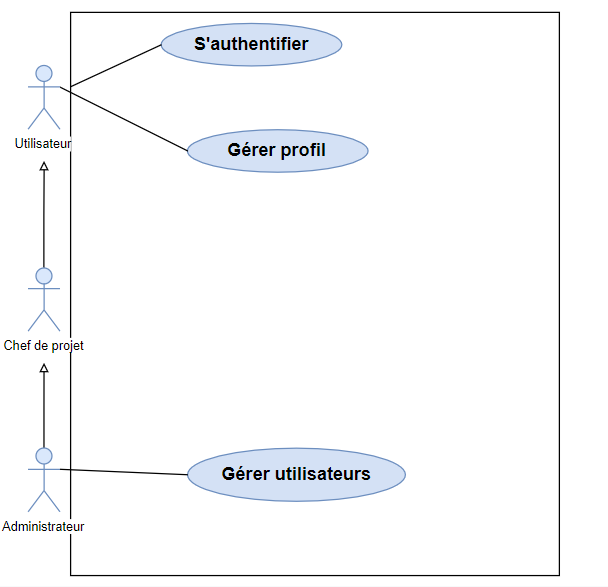
\includegraphics[scale=0.6]{Rsprint1.PNG}
	\caption{Diagramme de cas d'utilisation du sprint 1}
	\label{Diagramme de cas d'utilisation du sprint 1}
\end{figure} 
Comme le montre la figure 3.1, ce sprint permet aux utilisateur d'accéder facilement à l'application et de gérer leurs données personnelles sur leurs profils. Ainsi, pendant cette itération, l'administrateur devient capable de gérer tous les utilisateurs inscrits dans l'application.
\section{Gestion des comptes }

Cette partie est consacrée à la gestion des comptes personnels des utilisateurs. Ce dernier est composé  par les cas d'utilisation "s'authentifier" et "gérer profil". 
\subsection{Analyse}
Afin de mieux  détailler le fonctionnement et assimiler les cas d'utilisation de la première partie   constituant  ce sprint, nous allons établir, dans cette section,  leurs raffinements en livrant
une description sur les différents scénarios possibles.
\begin{itemize}
	\item \textbf{Raffinement du cas d'utilisation "S'authentifier"}\\
\end{itemize}

	\begin{figure}[H]
		\centering
		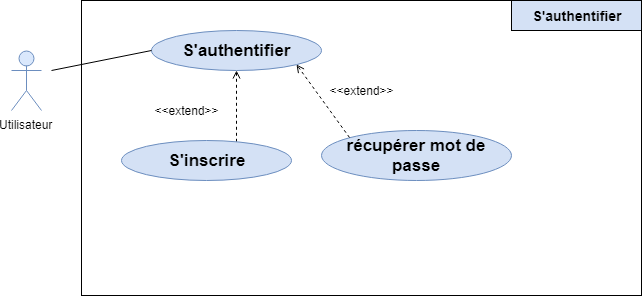
\includegraphics[scale=0.7]{Rauth.png}
		\caption{Raffinement du cas d'utilisation: S'authentifier}
		\label{Raffinement du cas d'utilisation: S'authentifier}
	\end{figure} 
Comme le montre la figure 3.2 un utilisateur peut soit s'authentifier ou bien créer un compte s'il s'agit d'un nouveau
utilisateur. L'application offre la possibilité de récupérer son mot de passe en cas d'oubli
en envoyant un nouveau mot de passe par émail.
Si l'utilisateur est authentifié avec succès, une page d'accueil sera ouverte, sinon, il sera
redirigé vers la page d'authentification.

 \textbf{Description textuelle du cas d'utilisation "Créer un compte"}

\begin{table}[H]
	\begin{tabular}{|l|l|}
		\hline
		\textbf{Acteur}                              & Utilisateur                                                                                                                                               \\ \hline
		\textbf{Description}                         & Ajouter un utilisateur au système.                                                                                                                        \\ \hline
		\textbf{Préconditions}                       & Disponibilité d'accès au serveur.                                                                                                                         \\ \hline
		\textbf{Post-conditions}                     & Utilisateur inscrit.                                                                                                                                      \\ \hline
		\multirow{4}{*}{\textbf{Scénario principal}} & \begin{tabular}[c]{@{}l@{}}1. L'utilisateur remplit le formulaire, valide reCAPTCHA\\ puis confirme.\end{tabular}                                         \\ \cline{2-2} 
		& 2. Le système  vérifie l'unicité de l'utilisateur.                                                                                                        \\ \cline{2-2} 
		& \begin{tabular}[c]{@{}l@{}}3. Le système génère un mot de passe aléatoire et l'envoie à \\ l'utilisateur par mail.\end{tabular}                           \\ \cline{2-2} 
		& 4.  Le système ajoute l'utilisateur .                                                                                                                     \\ \hline
		\textbf{Scénario altérnatif}                 & \begin{tabular}[c]{@{}l@{}}2.a Le système retourne un message d'erreur indiquant \\ l'existence d'un utilisateur avec des cordonnées pareil.\end{tabular} \\ \hline
	\end{tabular}

\caption{Description textuelle du << Créer un compte >> }
\label{Description textuelle du << Créer un compte >>}
\end{table}
\begin{itemize}
	\item  \textbf{Raffinement du cas d'utilisation "Gérer le profil"}
\end{itemize}
\begin{figure}[H]
	\centering
	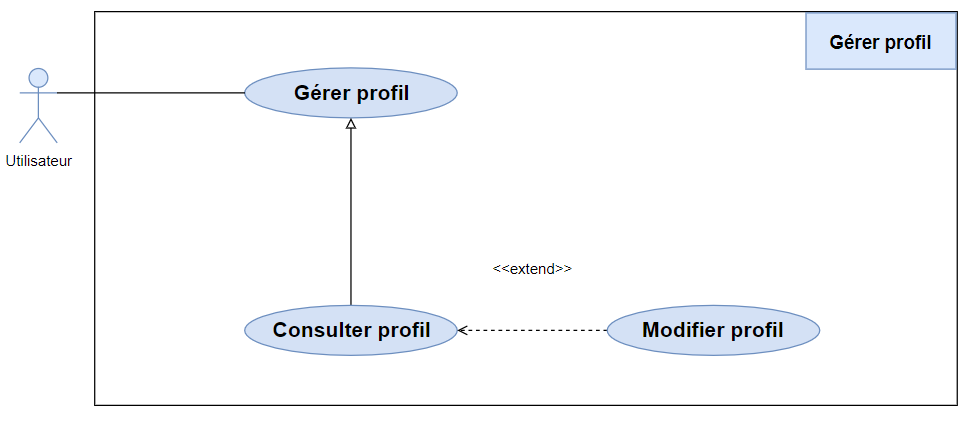
\includegraphics[ height=4cm, width=13cm]{Rprofil.PNG}
	\caption{Raffinement du cas d'utilisation:  Gérer le profil}
	\label{Raffinement du cas d'utilisation: Gérer le profil}
\end{figure} 

Le diagramme de cas d'utilisation de la figure 3.3  est une illustration des détails de la gestion du profil. En outre, ce diagramme montre la relation d'inclusion entre la consultation du profil et sa mise à jour.
\subsubsection{Description textuelle du sous cas d'utilisation: "Mettre à jour le profil"}

\begin{table}[ht]
	\begin{tabular}{|l|l|}
		\hline
		\textbf{Acteur}                               & Utilisateur.                                                                                                       \\ \hline
		\textbf{Description}                          & Mettre à jour profil.                                                                                              \\ \hline
		\textbf{Préconditions}                        & Utilisateur authentifié.                                                                                           \\ \hline
		\textbf{Post-conditions}                      & Profil mis à jour.                                                                                                 \\ \hline
		\multirow{5}{*}{\textbf{Scénario principal}}  & \begin{tabular}[c]{@{}l@{}}1. L'utilisateur clique sur  l'icône de mise à jour du profil.\end{tabular}           \\ \cline{2-2} 
		& 2. Le système afficher un formulaire.                                                                              \\ \cline{2-2} 
		& 3. L'utilisateur remplie le formulaire.                                                                            \\ \cline{2-2} 
		& 4. Le système met à jour le profil.                                                                                \\ \cline{2-2} 
		& 5.  Le système affiche le profil modifié.                                                                          \\ \hline
		\multirow{2}{*}{\textbf{Scénario altérnatif}} & \begin{tabular}[c]{@{}l@{}}3.a L'utilisateur laisse un champ vide, ou saisit de données\\ invalides.\end{tabular} \\ \cline{2-2} 
		& \begin{tabular}[c]{@{}l@{}}3.b Le système répond avec des messages d'erreurs.\end{tabular}                      \\ \hline
	\end{tabular}

\caption{Description textuelle du << Mettre à jour  le profil  >> }
\label{Description textuelle du << Mettre à jour le profil >>}
\end{table}


\subsection{Conception} 
Les diagrammes de séquence objet permettent de représenter les vues dynamiques du système en montrant les
collaborations entre les objets selon un point de vue temporel. Dans ce qui suit, nous allons
représenter les diagrammes de séquences les plus importants de la première partie de cette itération.\\
\textbf{Diagramme de séquences  du cas d'utilisation  "S'authentifier"}\\
\begin{figure}[H]
	\centering
	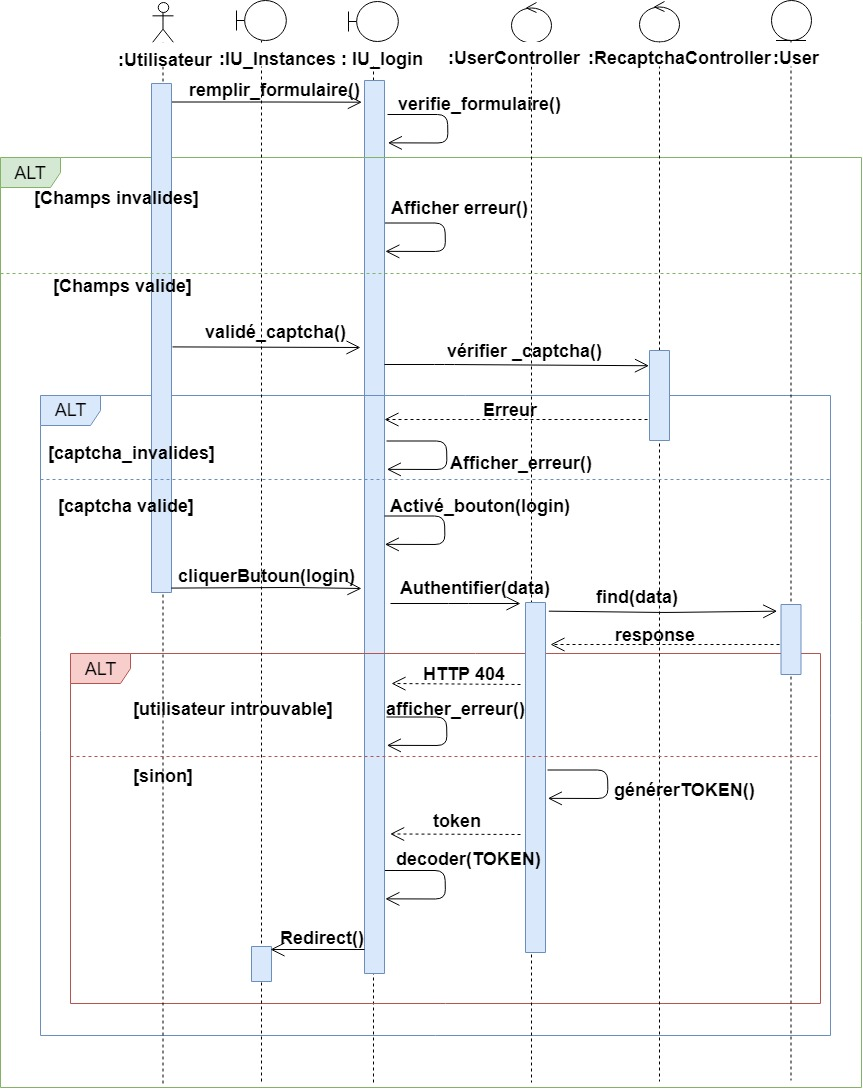
\includegraphics[scale=0.5]{login1.jpg}
	\caption{Diagramme de séquence: S'authentifier}
	\label{Diagramme de séquence: S'authentifier}
\end{figure} 

La figure 3.4  présentée ci dessous décrit la  procédure d'authentification à l'application. Tout d'abord,  l'utilisateur saisit son email et mot de passe. Une validation des champs se produit automatiquement, s'ils sont  invalides, un message d'erreur s'affiche, sinon  l'utilisateur continue sa procédure en validant recaptcha. Une fois validé et le bouton de connexion est appuyé,  les données s'envoient au contrôleur pour vérifier l'existence et la correspondance des coordonnées. Si c'est le cas, le contrôleur génère un token et l'émet pour qu'il soit décodé et utilisé dans l'envoie des prochaines requêtes, sinon il retourne une requête http portant le statut 401 indiquant la non autorisation d'accès.


\textbf{Diagramme de séquence du sous cas d'utilisation "Réinitialiser mot de passe"}\\
\begin{figure}[H]
	\centering
	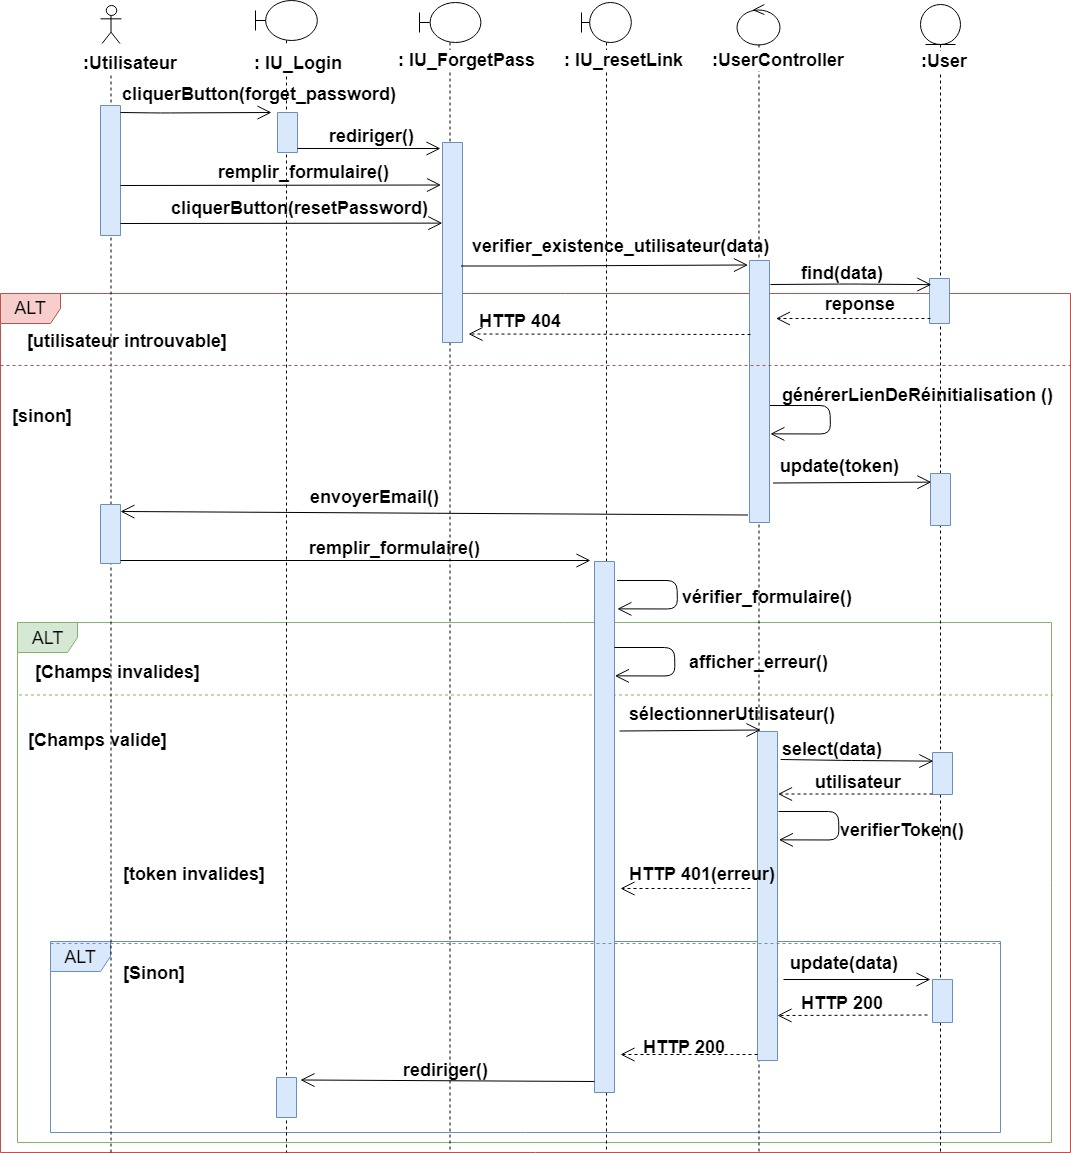
\includegraphics[scale=0.4]{resetpassword.jpg}
	\caption{Diagramme de séquence: Réinitialiser mot de passe}
	\label{Diagramme de séquence: Réinitialiser mot de passe}
\end{figure}

Le diagramme de la figure 3.5 ci dessus, met en évidence la procédure de  réinitialisation du mot de passe. Tout d'abord, l'utilisateur demande un nouveau mot de passe en appuyant sur le bouton correspondant. Ensuite, il sera redirigé vers l'interface de réinitialisation du mot de passe, là ou il devra saisir son email. Une fois son existence est validée, le contrôleur régénère un token et envoie un email contenant un lien de régénération du mot de passe.
L'utilisateur choisit alors un nouveau mot de passe et l'émet au contrôleur pour mettre à jour l'ancien token et l'ancien mot  de passe. Le contrôleur répond avec une requête HTTP de statut 200 si tout est bien. 

\subsubsection{Diagramme de séquence du cas d'utilisation: "Mettre à jour son profil"}

\begin{figure}[H]
	\centering
	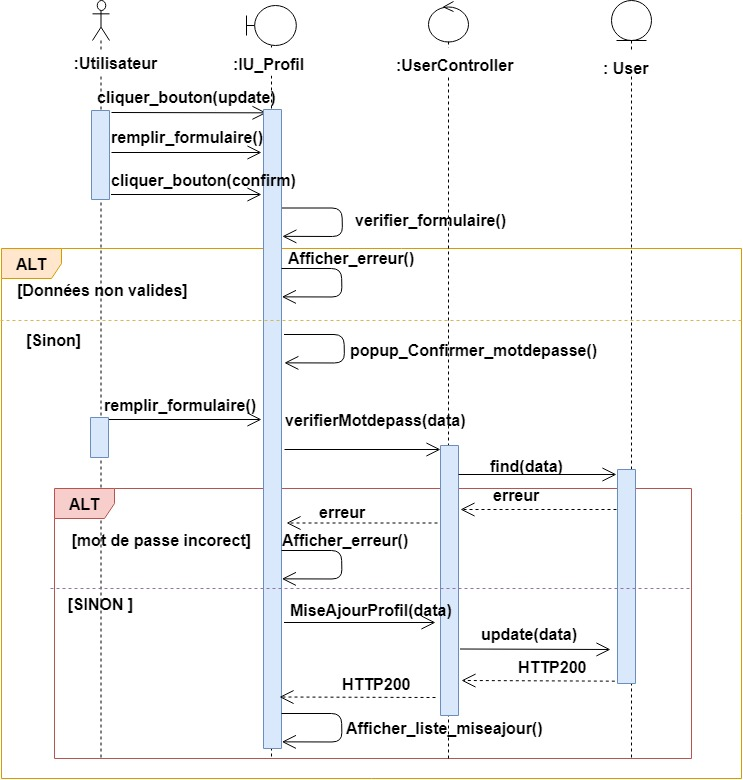
\includegraphics[height=11cm,width=14cm]{Majprofil-Page-1.jpg} 
	\caption{Diagramme de séquence: Mettre à jour profil}
	\label{Diagramme de séquence: Mettre à jour profil}
\end{figure}
Le diagramme de la figure 3.6 décrit la procédure de modification des données personnelles. En effet, l'utilisateur accède à son profil, là ou il clique sur l'icône d'activation de mode édition. Il saisit les données à modifier et  confirme sa modification en cliquant sur le bouton confirme. Une fois cliqué, une modale s'ouvre demandant de confirmer encore par le saisie du mot de passe. 
L'utilisateur saisit alors son mot de passe. Ce dernier est envoyé au contrôleur pour valider son existence. S'il est valide  les changements seront pris en compte et le contrôleur retourne une requête http de statut 200 sinon il retourne une requête de statut 401.

\section{Gestion des utilisateurs}
Cette partie est consacrée à la gestion des utilisateurs. Elle est composée  par le cas d'utilisation "gérer les utilisateurs". 
\subsection{Analyse}
Dans ce qui suit, nous allons offrir une vue d'ensemble des différentes fonctionnalités relatives à la deuxième partie de ce sprint. Ensuite, nous allons raffiner et décrire
les cas d'utilisation les plus prioritaires.
\subsubsection{Raffinement du cas d'utilisation: "Gérer utilisateurs" }
\begin{figure}[H]
	\centering
	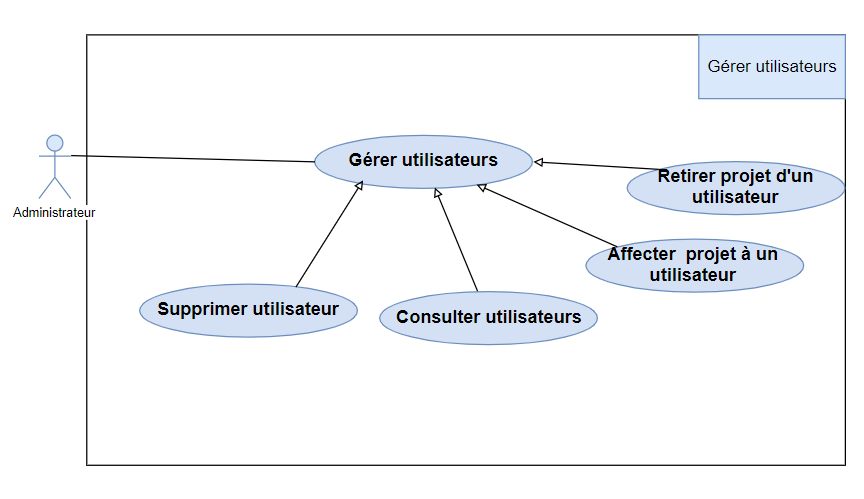
\includegraphics[ height=4.8cm, width=14cm]{Rgererusers.PNG}
	\caption{Raffinement du cas d'utilisation: Gérer les utilisateurs}
	\label{Raffinement du cas d'utilisation: Gérer les utilisateurs}
\end{figure}
Le diagramme de la figure 3.7 présente un raffinement relatif au cas d'utilisation "gérer les utilisateurs". En effet, à travers la consultation de la liste des utilisateurs nous pouvons  soit supprimer, soit affecter un projet à un utilisateur ou bien retirer un projet de l' utilisateur.
\subsubsection{Description textuelle du sous cas d'utilisation: "Supprimer un utilisateur"}

% Please add the following required packages to your document preamble:
% \usepackage{multirow}
\begin{table}[H]
	\begin{tabular}{|l|l|}
		\hline
		\textbf{Acteur}                               & Administrateur.                                                                                                                                             \\ \hline
		\textbf{Description}                          & Supprimer un compte utilisateur du système.                                                                                                                 \\ \hline
		\textbf{Préconditions}                        & Administrateur authentifié.                                                                                                                                 \\ \hline
		\textbf{Post-conditions}                      & Utilisateur supprimé.                                                                                                                                       \\ \hline
		\multirow{5}{*}{\textbf{Scénario principal}}  & \begin{tabular}[c]{@{}l@{}}1. L'administrateur clique sur l'icône de \\ suppression.\end{tabular}                                                           \\ \cline{2-2} 
		& 2. . Le système affiche une modale de confirmation.                                                                                                         \\ \cline{2-2} 
		& 3. L'administrateur clique sur confirme son choix.                                                                                                          \\ \cline{2-2} 
		& \begin{tabular}[c]{@{}l@{}}4. Le système supprime l'utilisateur correspondant et affiche \\ un message manifestant la réussite de l'opération.\end{tabular} \\ \cline{2-2} 
		& 5. Le système affiche la nouvelle liste des utilisateurs.                                                                                                   \\ \hline
		\multirow{2}{*}{\textbf{Scénario altérnatif}} & \begin{tabular}[c]{@{}l@{}}2.a L'administrateur décide d'annuler l'opération de \\ suppression.\end{tabular}                                                \\ \cline{2-2} 
		& \begin{tabular}[c]{@{}l@{}}2.b Le système ferme la modale et affiche la liste des\\ utilisateurs mise à jour.\end{tabular}                                  \\ \hline
	\end{tabular}

\caption{Description textuelle du << Supprimer un utilisateur >> }
\label{Description textuelle du << Supprimer un utilisateur >>}
\end{table}
% Il faut ajouter que il peut chercher un utilisateur inexistant
\subsection{Conception}
Afin de décortiquer et détailler les cas d'utilisation précédemment cités, nous présentons dans ce qui suit les diagrammes de séquences des cas d'utilisation les plus importants
\subsubsection{Diagramme de séquence du cas d'utilisation: "Supprimer un utilisateur"}

\begin{figure}[H]
	\centering
	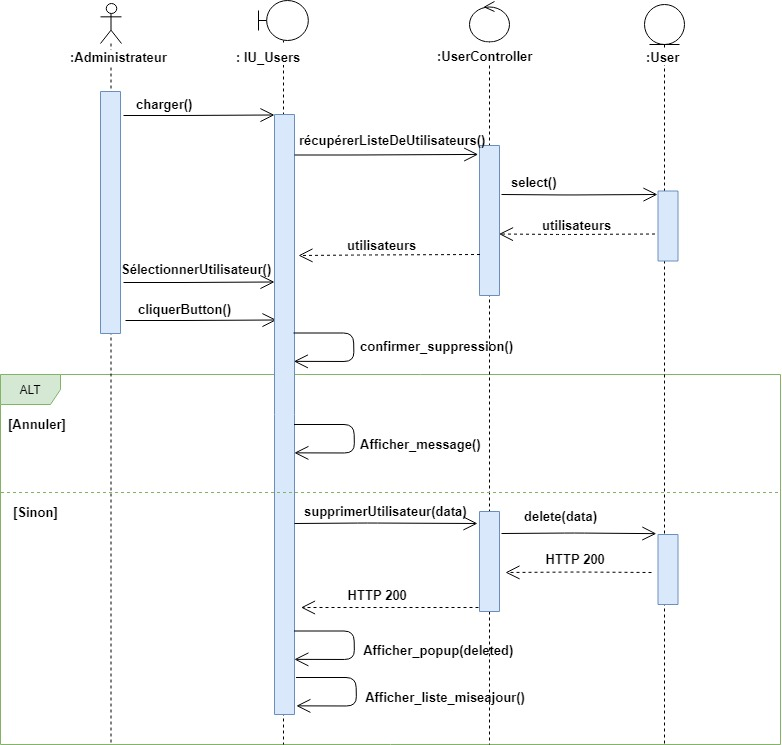
\includegraphics[scale=0.55]{deleteuser.jpg}
	\caption{Diagramme de séquence: Supprimer un utilisateur}
	\label{Diagramme de séquence: Supprimer un utilisateur}
\end{figure}
Le diagramme de la figure 3.8 décrit l'opération de suppression d'un utilisateur. Tout d'abord, l'administrateur accède à la liste des utilisateurs. Ensuite, 
Il clique sur le bouton de suppression correspondant. Une fois cliqué, une modale de confirmation s'ouvre. Là ou il peut soit annuler l'opération, soit la confirmer. S'il appuie sur le bouton de confirmation  les données nécessaires à la suppression seront émises au contrôleur pour 
vérifier l'existence de l'utilisateur à partir de son email. Par la suite, le contrôleur retourne une requête http de statut 200, dans le cas ou l'utilisateur existe. Il retourne une erreur, dans le cas contraire.


\section{Réalisation}
\subsection{Sécurité}
\begin{itemize}
	\item \textbf{Authentification avec reCAPTCHA}: Permettant de vérifier l'identité annoncée, s'assurer de la non usurpation d'identité de la personne en question, empêcher les accès  automatisés par les robots et   toute tentative de spam.
	\item \textbf{Autorisation}: Permettant la vérification de privilèges de chaque utilisateur pour accéder à la ressource demandée.Dans Symfony 4, il s'agit d'un fichier de configuration  "Security.yaml"  réparti en sections dont chaque section assure un role bien important dans la sécurité 
	\begin{itemize}
		\item Section "firewalls" met en évidence la méthode d'authentification elle peut être soit par login et mot de passe, soit par la méthode HTTP ou bien à travers un compte de réseau social.
		\item Section "access control"  permet de gérer les droits d'accès des utilisateurs.
		\item Section "encoders" permet de spécifier l'algorithme de hashage  à utiliser pour stocker le mot de passe.
	\end{itemize} 
\item \textbf{Cryptage des mots de passe}: 
Pour se protéger contre les attaques et assurer la confidentialité et  l'intégrité des mots de passe des utilisateurs, nous avons opté pour le chiffrement de ses derniers par  l'algorithme "argon2i" à travers la section "encoders" de fichier "Security.yaml" de Symfony.
\item \textbf{Sécurisation des APIs}: L'échange des informations concernant l'utilisateur couramment authentifié est sécurisé au moyen des jetons JWT pour (Json Web Token) généré par le serveur.

 \textbf{Structure de JWT} \\Ce standard de transmission des informations est composé de trois parties définies par la figure 3.5. 



	\begin{itemize}
	\item Header: contient le type de jeton et l'algorithme utilisé pour la signature.
	\item Payload: contient toutes les données personnelles de l'utilisateur.
	\item Signature:  hachage d'en-tête, de charge utile de la partie Payload et d'une clé secrète codée.
	 	
\end{itemize}
	\begin{figure}[H]
	\centering
	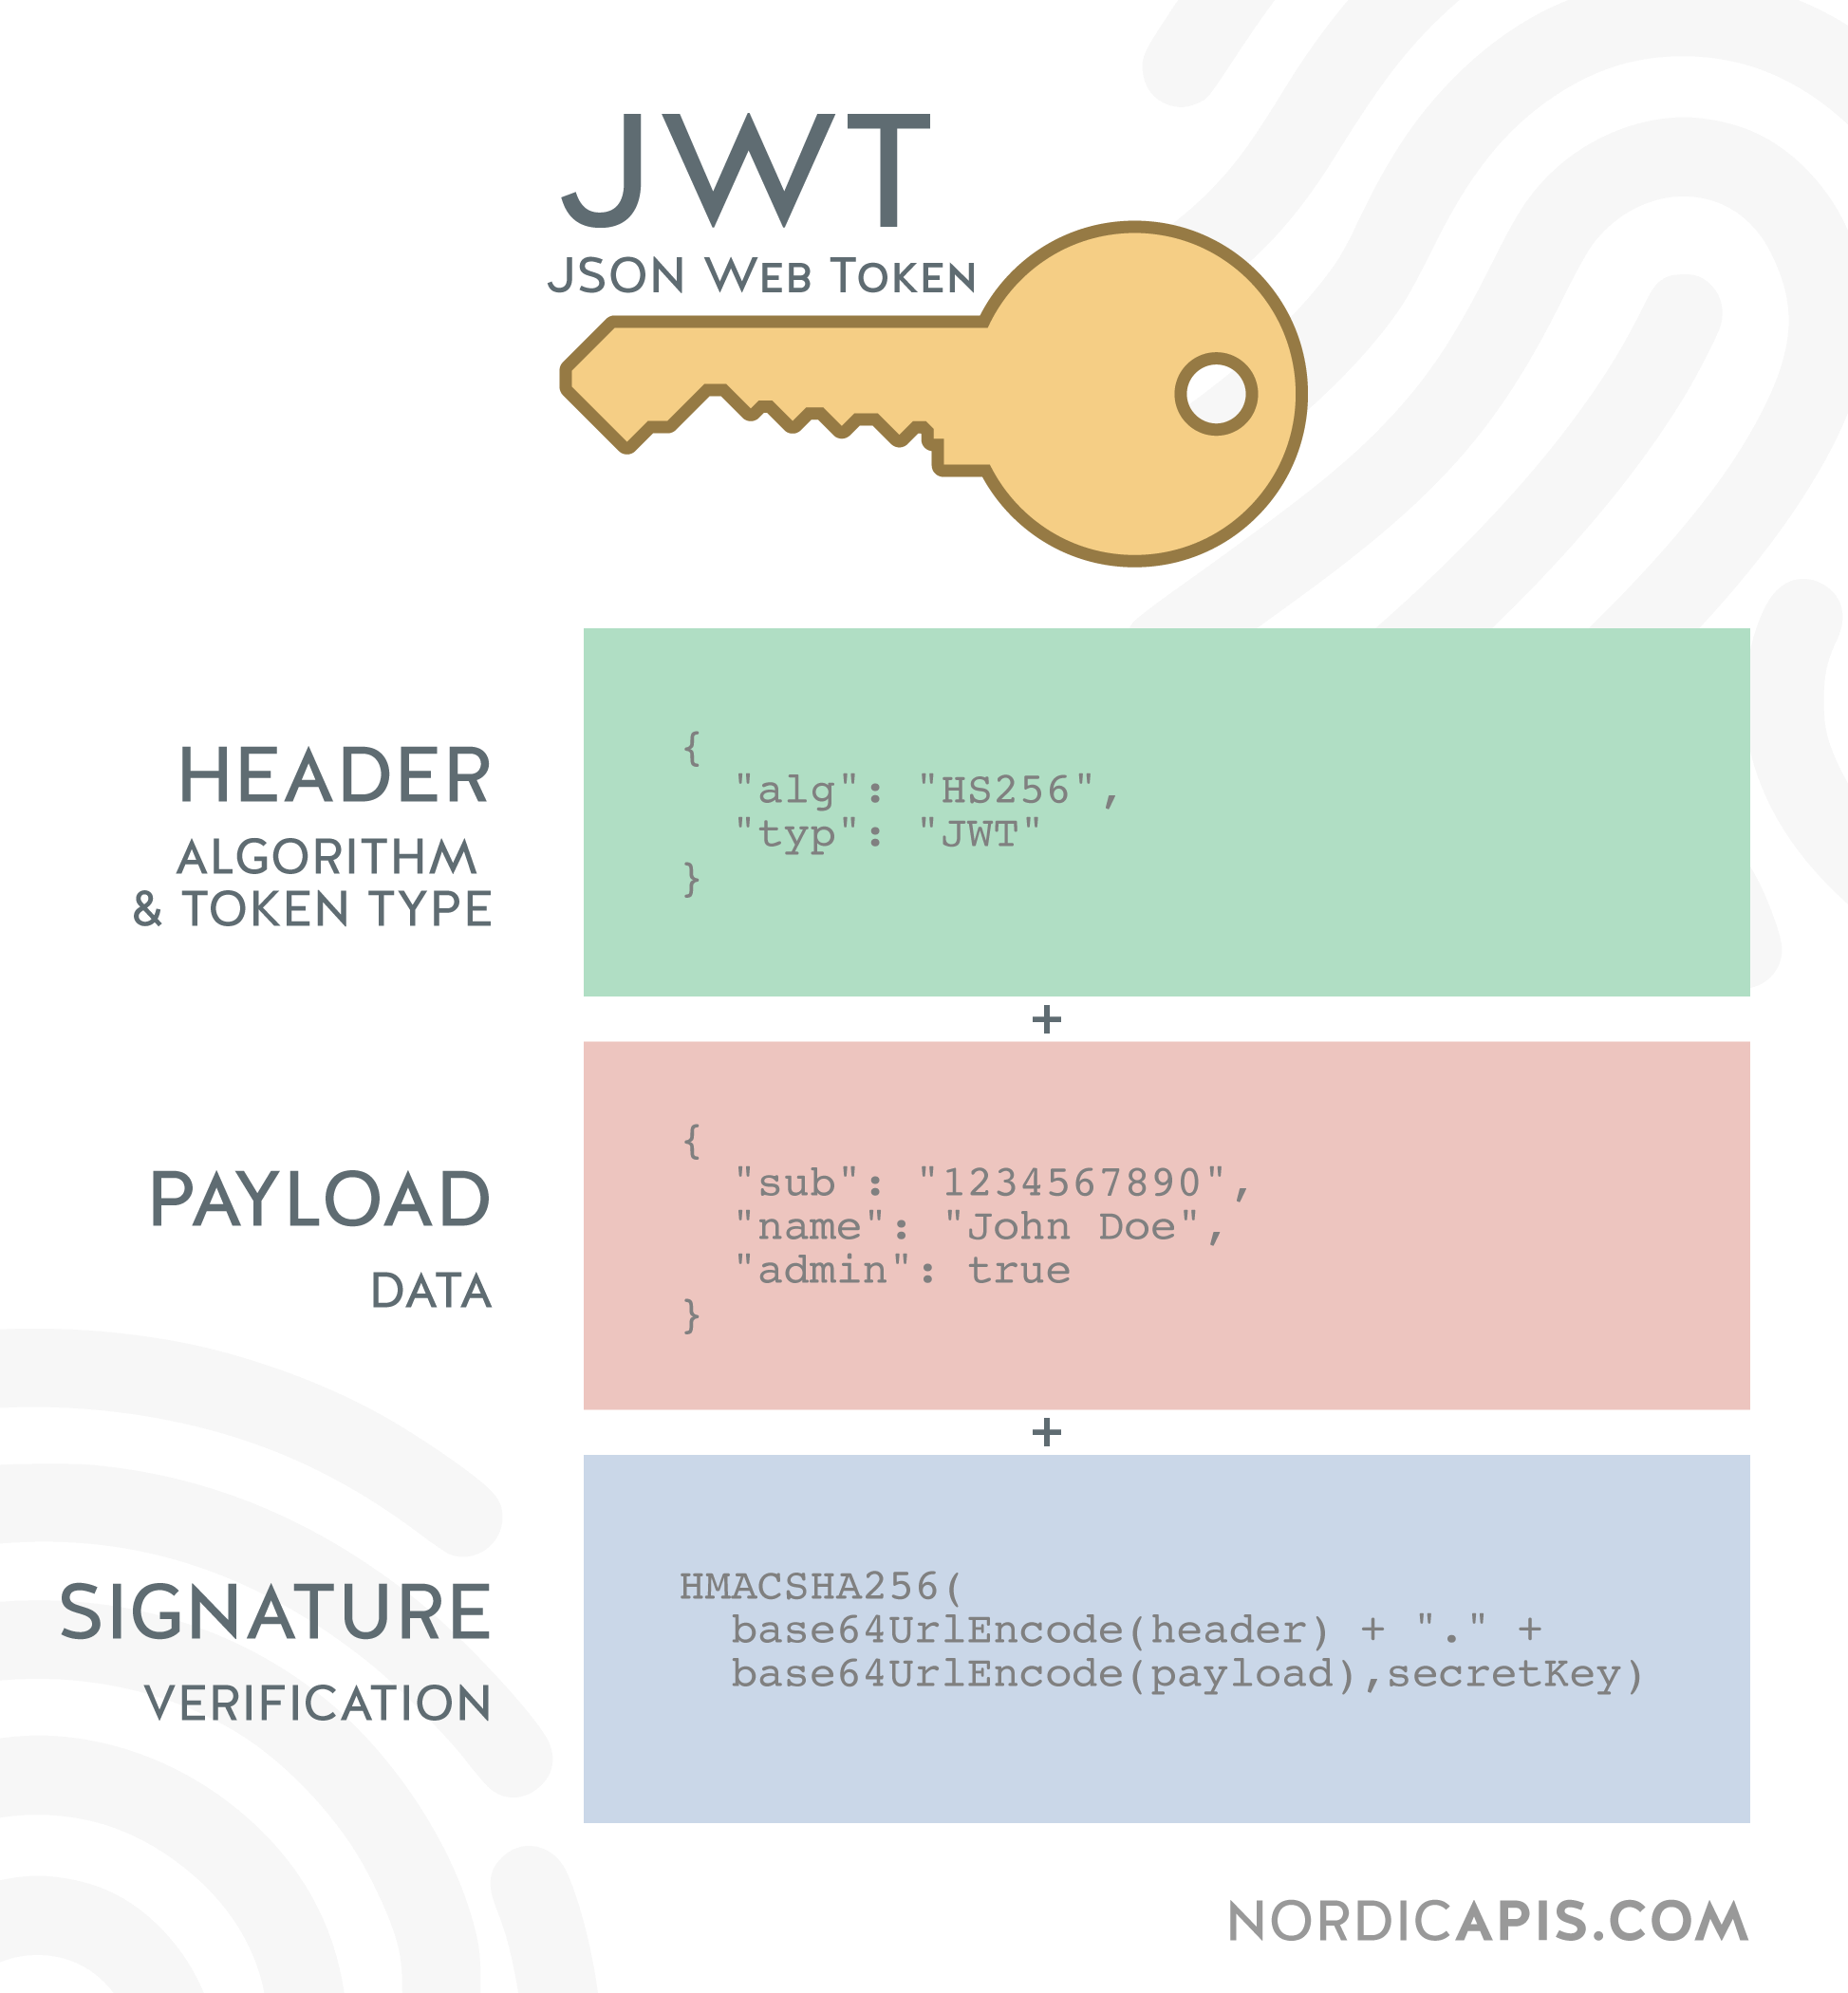
\includegraphics[scale=0.09]{jwt2.png}
	\caption{Structure de JWT}
	\label{Structure de JWT}
\end{figure} 
\newpage
\textbf{Fonctionnement de JWT}
	\begin{figure}[H]
	\centering
	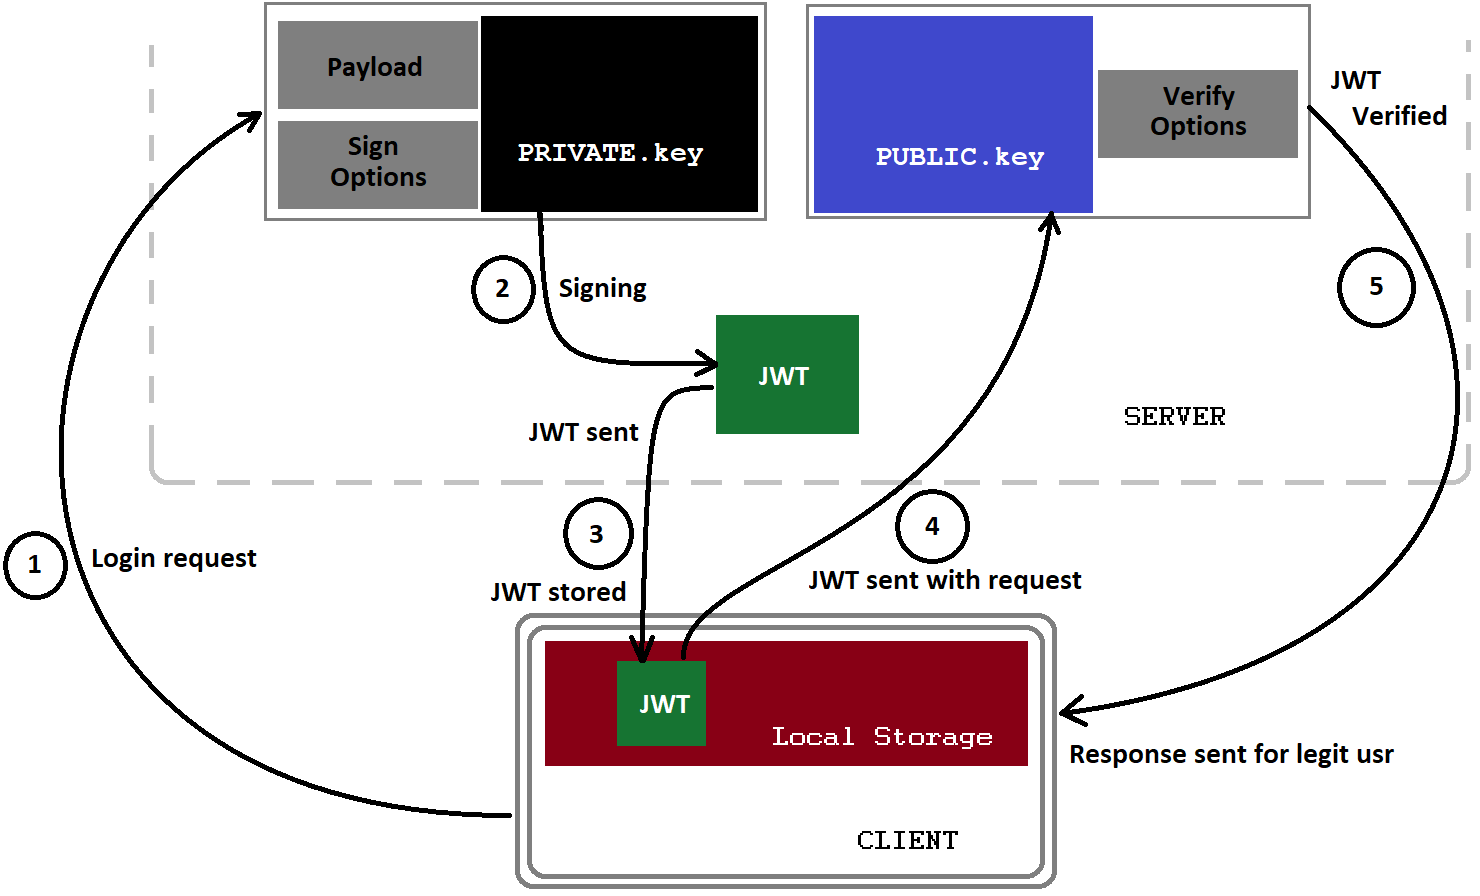
\includegraphics[scale=0.2]{jwt.png}
	\caption{Fonctionnement de JWT}
	\label{Fonctionnement de JWT}
\end{figure} 

Comme présenté par la figure 3.10 lorsqu'un utilisateur envoie une requête avec les paramètres requis tels que le mail d'utilisateur et
son mot de passe. L'application vérifie si le mail d'utilisateur et le mot de passe sont valides. Lors de
la validation, l'application créera un jeton à l'aide d'un payload et d'une clé secrète. Il renverra
ensuite le jeton à l'utilisateur pour l'enregistrer à "local storage" et l'envoyer à chaque demande. Lorsque l'utilisateur
envoie une requête avec ce jeton, l'application vérifie la validité avec la même clé secrète. Si le
jeton est valide, la demande est envoyée, sinon l'application enverra un message d'erreur approprié.



\end{itemize}
\subsection{Interfaces}
Nous montrons le résultat du sprint courant,dans la partie qui suit, à travers des imprimes écran.
\begin{figure}[!htb]
	\minipage{0.4\textwidth}
	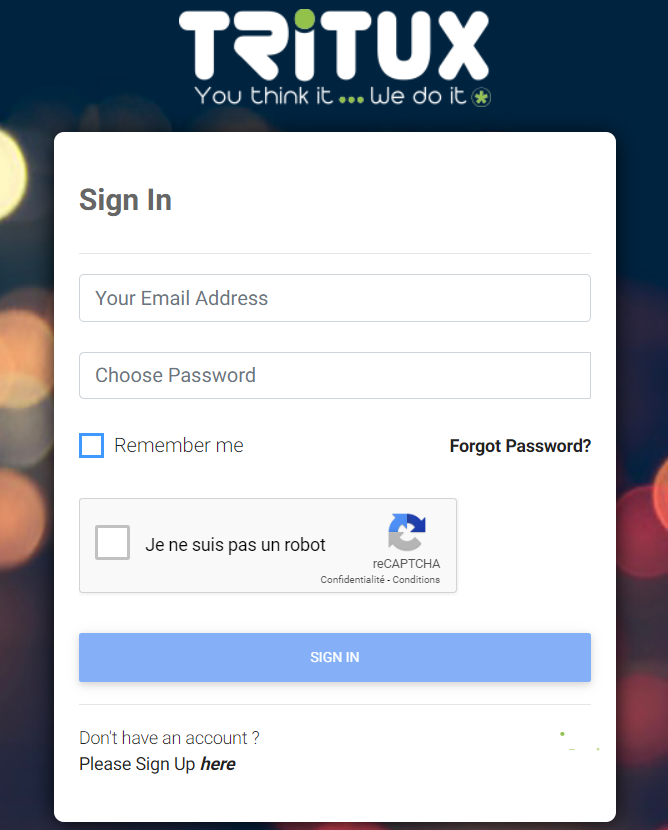
\includegraphics[width=\linewidth, height=7.3cm]{login.PNG}
	\caption{Interface de connexion à l'application }\label{fig:Interface de connexion à l'application }
	\endminipage\hfill
	\minipage{0.4\textwidth}
	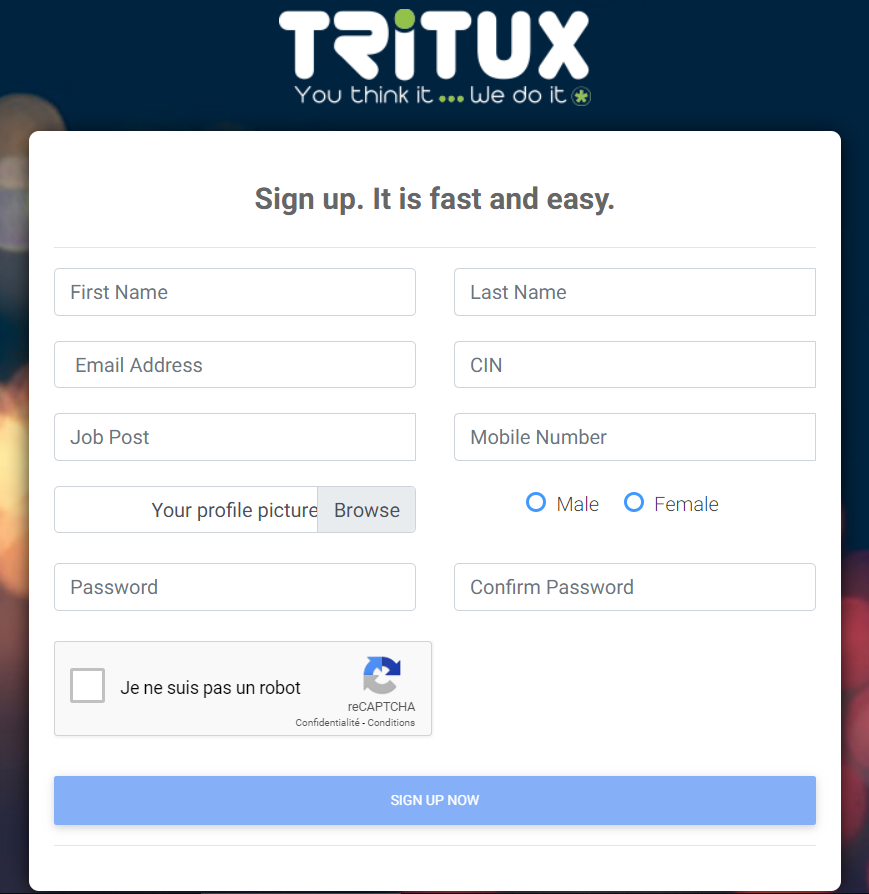
\includegraphics[width=\linewidth,height=7.5cm]{inscription.PNG}
	\caption{Interface d'inscription}\label{fig:Interface d'inscription }
	\endminipage\hfill
\end{figure}

La figure 3.11 montre l'interface de l'ouverture de l'application. Si un utilisateur ne possède pas de compte il peut s'inscrire à travers la figure 3.12  ou  bien s'il est déjà inscrit mais il a oublié son mot de passe, il peut le réinitialiser à travers les interfaces décrites dans les figures 3.13 et 3.14.

\begin{figure}[!htb]
	\minipage{0.4\textwidth}
	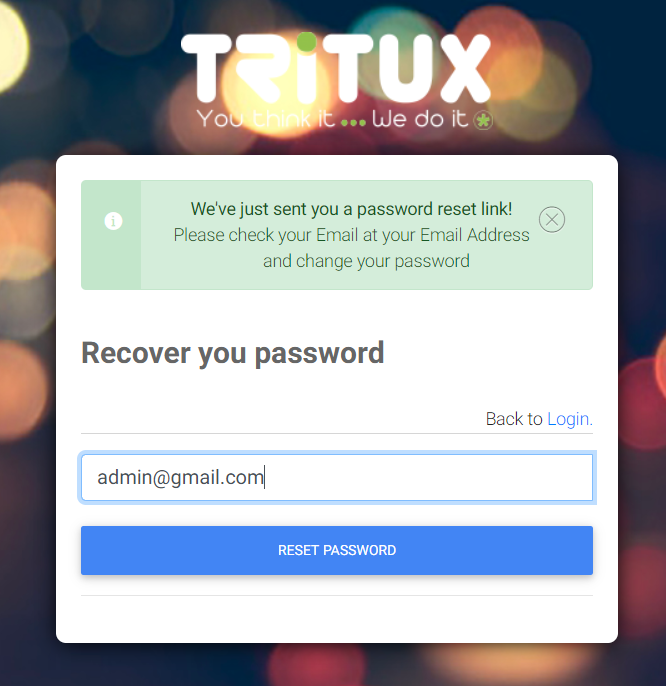
\includegraphics[width=\linewidth, height=7.4cm]{reinitmdp.PNG}
	\caption{Interface de réinitialisation du mot de passe }\label{fig: Interface de réinitialisation du mot de passe }
	\endminipage\hfill
	\minipage{0.4\textwidth}
	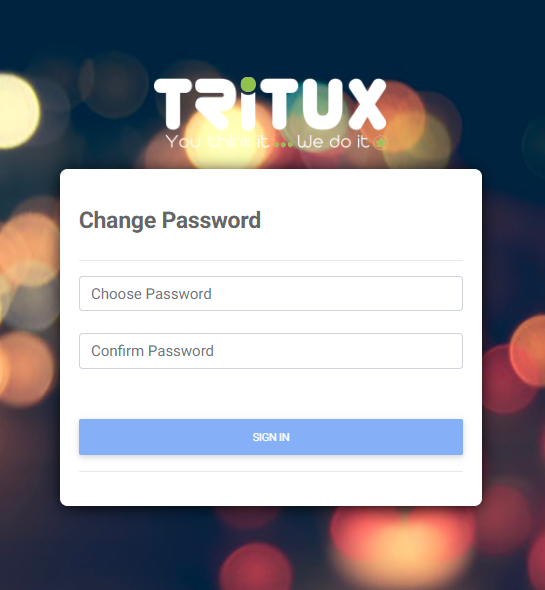
\includegraphics[width=\linewidth, height=7cm]{recoverpass1.PNG}
	\caption{Interface d'affectation d'un nouveau mot de passe en cas d'oubli}\label{fig:Interface d'affectation d'un nouveau mot de passe en cas d'oubli}
	\endminipage\hfill
\end{figure}

\begin{figure}[H]
\centering
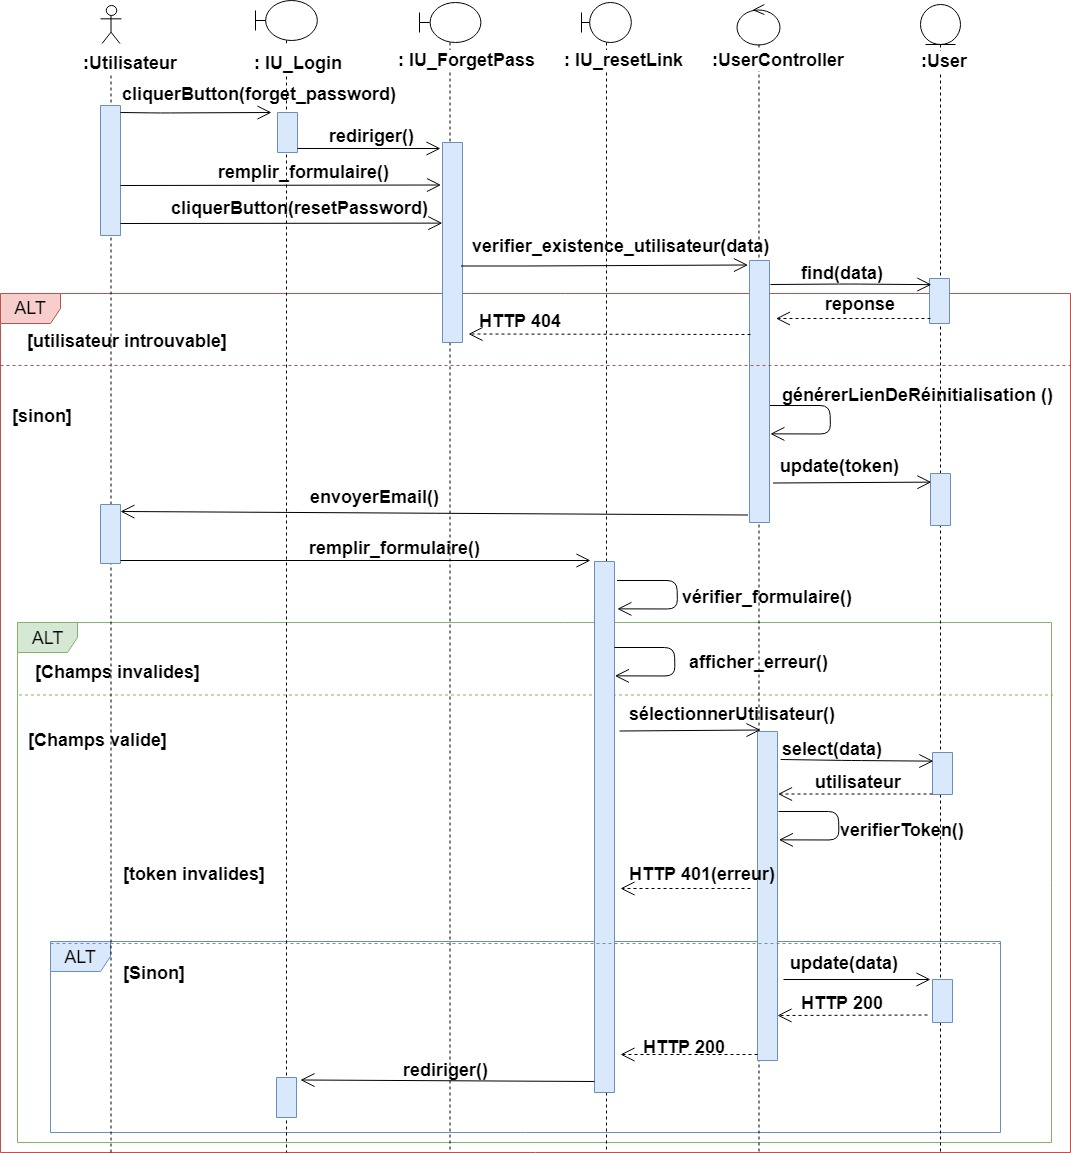
\includegraphics[height=10cm,width=15cm]{resetpassword.jpg}
\caption{ Email de réinitialisation du mot de passe }
\label{Email de réinitialisation du mot de passe}
\end{figure}
La figure 3.15 représente l'interface de gestion du profil. Dedans l'utilisateur aura la possibilité de modifier ses données personnelles comme le montre la figure 3.16.


	\begin{figure}[H]
	\centering
	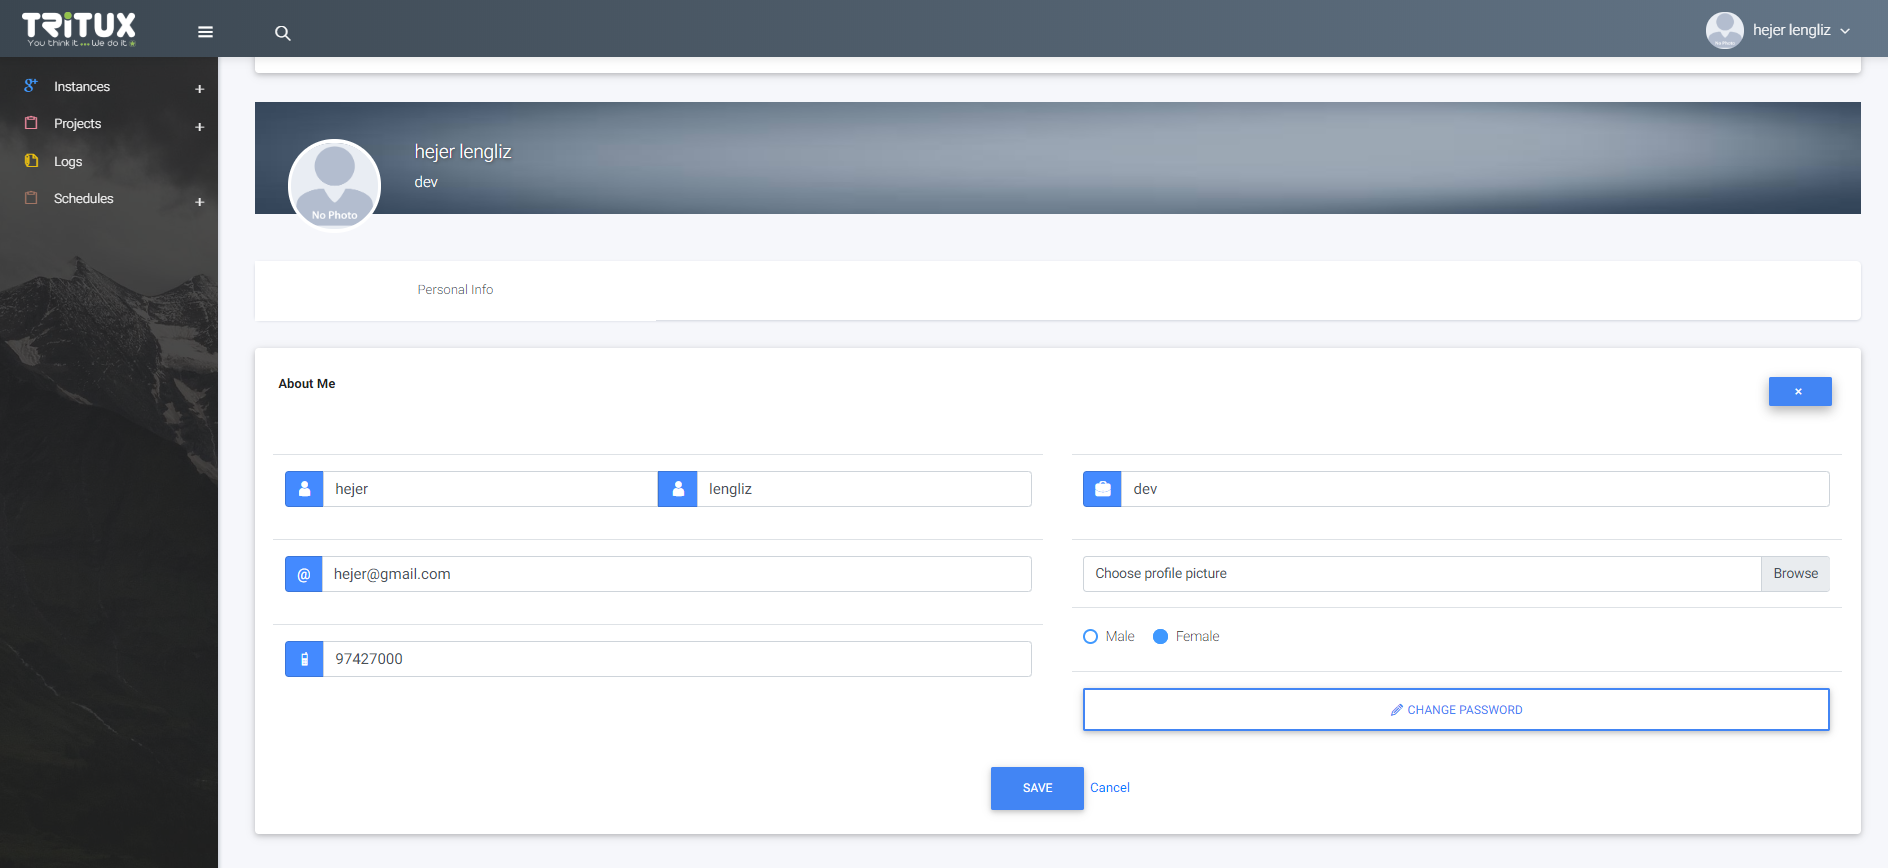
\includegraphics[scale=0.35]{editprofile.PNG}
	\caption{Interface de mise à jour du profil}
	\label{Interface de mise à jour du profil}
\end{figure}
	\begin{figure}[H]
	\centering
	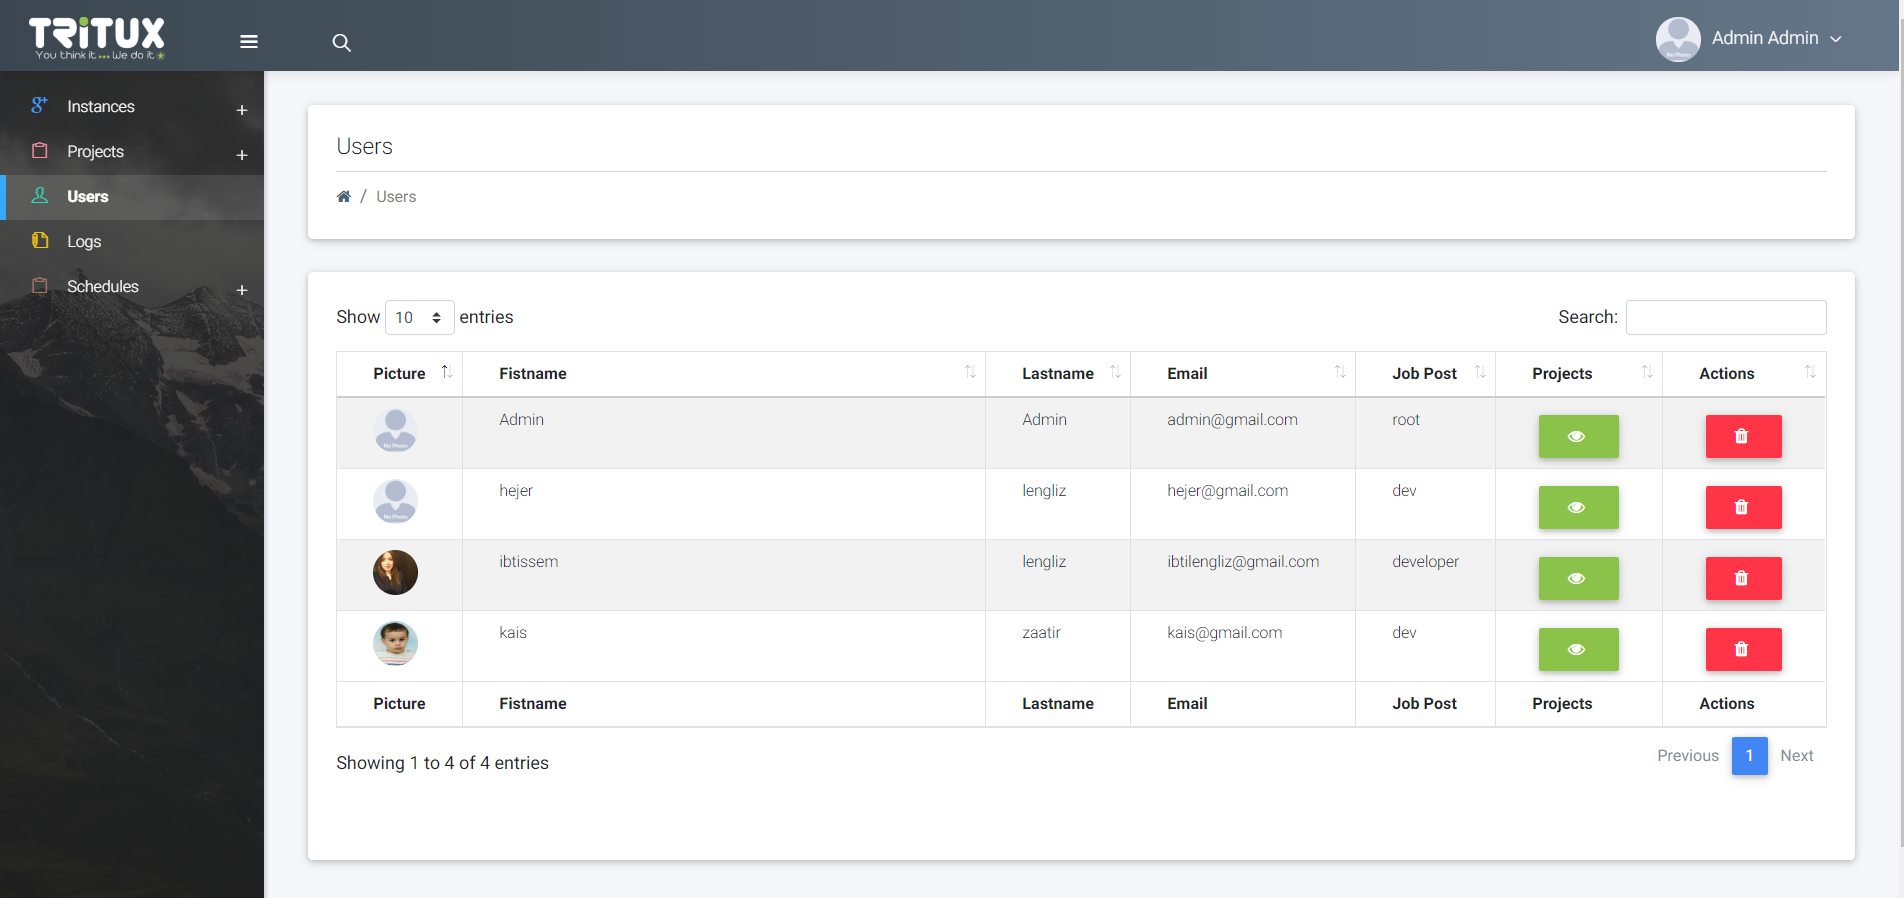
\includegraphics[scale=0.35]{users.PNG}
	\caption{Interface de gestion des utilisateurs}
	\label{Interface de gestion des utilisateurs}
\end{figure}
La figure 3.16 représente l'interface de gestion des utilisateurs, grâce à laquelle l'administrateur
pourra rechercher , supprimer un utilisateur et  affecter ou retirer un projet de l'utilisateur.


\section{Conclusion}
Le résultat d'un sprint est un produit livrable au client. Tout au long de ce chapitre,
nous avons réussi à produire un incrément ayant suffisamment de valeur pour le client
et pourra être utilisé dans un environnement de production. Dans le chapitre qui suit,
notre effort sera consacré pour produire une nouvelle valeur métier couvrant les fonctionnalités
de management des projets et des machines virtuelles.
